Un loueur de bicyclettes propose deux types de bicyclettes : des bicyclettes traditionnelles et des bicyclettes électriques. Il incite ses clients à prendre une assurance. On dispose des informations suivantes.
\begin{itemize}[label=$\bullet$]
	\item 60\% des clients ont loué une bicyclette traditionnelle, les autres ont loué une bicyclette électrique.
	\item Parmi ceux qui ont loué une bicyclette traditionnelle, 25\% ont pris une assurance.
	\item 20\% de l'ensemble des clients ont pris une assurance.
\end{itemize}

On choisit un client au hasard et on note les événements :

\textit{T} : \og{}le client a loué une bicyclette traditionnelle\fg{}.

\textit{A} : \og{}le client a pris une assurance\fg{}.

\begin{enumerate}
	\item Recopier l'arbre pondéré ci-dessous et compléter les pointillés.


\begin{center}
			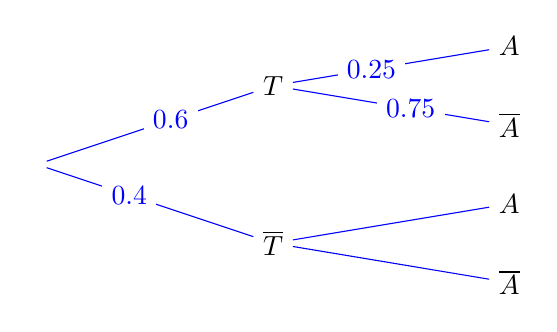
\begin{tikzpicture}[xscale=1,yscale=1,rotate=0,every node/.style={scale=1,rotate=0}]
			\node(n0)at(0,0){};
			\node(n1_1)at(3,1){$T$};
			\node(n1_2)at(3,-1){$\overline{T}$};
			\node(n2_1)at(6,1.5){$A$};
			\node(n2_2)at(6,0.5){$\overline{A}$};
			\node(n2_3)at(6,-0.5){$A$};
			\node(n2_4)at(6,-1.5){$\overline{A}$};
			\draw[blue](n0)--(n1_1)node[pos=0.6,fill=white]{\np{0.6}};
			\draw[blue](n0)--(n1_2)node[pos=0.4,fill=white]{\np{0.4}};
			\draw[blue](n2_1)--(n1_1)node[pos=0.6,fill=white]{\np{0.25}};
			\draw[blue](n2_2)--(n1_1)node[pos=0.4,fill=white]{\np{0.75}};
			\draw[blue](n2_3)--(n1_2);
			\draw[blue](n2_4)--(n1_2);

		\end{tikzpicture}

\end{center}
		\item Donner, par simple lecture de l'énoncé, la probabilité de l'événement A.


		 \textcolor{red}{\textsc{Correction}}


		20\% des clients ont pris l'assurance, donc \mbox{$P(A)=\np{0.2}$}
		\item Montrer que la probabilité que le client ait loué une bicyclette traditionnelle et qu'il ait pris une assurance est égale à \np{0.15}.

		 \textcolor{red}{\textsc{Correction}}


		\mbox{$P(T \cap A)=P(T)\times P_T(A)=\np{0.6}\times\np{0.25}=\np{0.15}$}.

		\item En déduire que la probabilité \mbox{$P(\overline{T}\cap A)$} est égale à \np{0.05}.

		 \textcolor{red}{\textsc{Correction}}


		Loi des probabilités totales : \quad \mbox{$P(A)=P(T\cap A)+P(\overline{T}\cap A)$};

		donc \mbox{$P(\overline{T}\cap A)=P(A)-P(T\cap A)=\np{0.2}-\np{0.15}=\np{0.05}$}

		la probabilité qu'un client ait loué une bicyclette électrique et pris une assurance est \np{0.05}.

		\item Déterminer la probabilité que le client ait pris une assurance sachant qu'il a loué une bicyclette électrique. On donnera le résultat sous la forme d'une fraction irréductible.

			 \textcolor{red}{\textsc{Correction}}


		Puisque \quad \mbox{$P(\overline{T}\cap A)=P(\overline{T})\times P_{\overline{T}}(A)$},

		On en déduit :\quad \mbox{$P_{\overline{T}}(A)=\dfrac{P(\overline{T} \cap A)}{P(\overline{T})} = \dfrac{\np{0.05}}{\np{0.4}}=\dfrac18$}

		la probabilité qu'un client ayant loué une bicyclette électrique ait pris une assurance est \mbox{$\dfrac18=\np{0.125}$}

\end{enumerate}
